\chapter{Numerische berechnung der Koeffizienten} \label{anh:Programm}
Hier wird nun ein Haskell Programm, dass in der Funktion \textbf{main} die
Koeffizienten von $v$ und $u$ numerisch berechnet. Wir wählen $a=\frac{1}{8}$,
dadurch gilt $u_{-2}=i$.
\lstinputlisting[language=HaskellUlisses]{../haskell/programm.hs}

Ist der Code in einer Datei \textbf{/Pfad/zu/koeff.hs} gespeicher, so lässt er
sich in Unix-Artigen Systemen beispielsweise mit den folgenden Befehlen
compilieren und ausführen.
\begin{lstlisting}[style=Bash]
$ ghc /Pfad/zu/koeff.hs
$ /Pfad/zu/koeff 15 20 30 40 50 100 150
\end{lstlisting}
Durch das Ausführen berechnet das Programm die Koeffizienten von $v$ und $u$
bis zum Index $15$ sowie einzelne Werte an $20$, $30$, $40$, $50$, $100$ und
$150$ und produziert einen Ausgang, der wie folgt aussieht
\begin{lstlisting}[style=Bash]
n       | v_n   u_n
--------+-----------------------------------------------
-2      | 0.0 :+ 0.0    0.0 :+ 1.0
-1      | 0.5 :+ 0.0    (-1.5) :+ (-0.0)
0       | 0.0 :+ (-0.75)    (-0.0) :+ 0.75
1       | (-1.5) :+ (-0.0)    1.5 :+ 0.0
2       | 0.0 :+ 3.9375    (-0.0) :+ (-3.9375)
3       | 13.5 :+ 0.0    (-13.5) :+ (-0.0)
4       | 0.0 :+ (-59.34375)    (-0.0) :+ 59.34375
5       | (-324.0) :+ (-0.0)    324.0 :+ 0.0
6       | 0.0 :+ 2122.98046875    (-0.0) :+ (-2122.98046875)
7       | 16213.5 :+ 0.0    (-16213.5) :+ (-0.0)
8       | 0.0 :+ (-141115.447265625)    (-0.0) :+ 141115.447265625
9       | (-1376311.5) :+ (-0.0)    1376311.5 :+ 0.0
10      | 0.0 :+ 1.4850124677246094e7    (-0.0) :+ (-1.4850124677246094e7)
11      | 1.75490226e8 :+ 0.0    (-1.75490226e8) :+ (-0.0)
12      | 0.0 :+ (-2.2530628205925293e9)    (-0.0) :+ 2.2530628205925293e9
13      | (-3.1217145174e10) :+ (-0.0)    3.1217145174e10 :+ 0.0
14      | 0.0 :+ 4.641652455250599e11    (-0.0) :+ (-4.641652455250599e11)
15      | 7.3709524476135e12 :+ 0.0    (-7.3709524476135e12) :+ (-0.0)
20      | 0.0 :+ (-1.753906248830001e19)    (-0.0) :+ 1.753906248830001e19
30      | 0.0 :+ 2.7520294973343126e33    (-0.0) :+ (-2.7520294973343126e33)
40      | 0.0 :+ (-1.1055855646065139e49)    (-0.0) :+ 1.1055855646065139e49
50      | 0.0 :+ 5.0878905001062135e65    (-0.0) :+ (-5.0878905001062135e65)
100     | 0.0 :+ (-3.045728894141079e159)    (-0.0) :+ 3.045728894141079e159
150     | 0.0 :+ 2.7737283214890534e264    (-0.0) :+ (-2.7737283214890534e264)
\end{lstlisting}
In Haskell ist das \textbf{:+} ein Infix-Konstruktor der Klasse
\textbf{Data.Complex}. So erzeugt ein Aufruf der Form \textbf{a :+ b} eine
Imaginärzahl, die $a+ib$ entspricht.

Übersetzt in unsere Zahlenschreibweise sieht das Ergebnis also wie folgt aus:

\begin{table}[htbp]
\begin{center} \scriptsize
\begin{tabular}{|r||r|r||r|}
\hline
n        & $v_n$                             & $u_n$ & Analytisch: $v_n$
\\\hline\hline
-2       & $0$                               & $i$ & $0$
\\-1     & $0,5$                             & $-1,5 $ & $\frac{1}{2}$
\\0      & $-0,75i$                          & $0,75i$ & $\neq\frac{3}{8a}i=\frac{3}{4}i$
\\1      & $-1,5$                            & $1,5$ & $\frac{3}{16a}=1,5$
\\2      & $3,9375i$                         & $-3,9375i$ & $\frac{-63i}{256a\sqrt{2a}} \approx -3.9375i$
\\3      & $13,5$                            & $-13,5$ &
\\4      & $-59,34375i$                      & $59,34375i$ &
\\5      & $-324,0$                          & $324,0$ &
\\6      & $2122,98046875i$                  & $-2122,98046875i$ &
\\7      & $16213,5$                         & $-16213,5$ &
\\8      & $-141115,447265625i$              & $141115,447265625i$ &
\\9      & $-1376311,5$                      & $1376311,5$ &
\\10     & $1,4850124677246094\cdot10^7i$    & $-1,4850124677246094\cdot10^7i$
&
\\11     & $1,75490226\cdot10^8$             & $-1,75490226\cdot10^8$ &
\\12     & $-2,2530628205925293\cdot10^9i$   & $2,2530628205925293\cdot10^9i$ &
\\13     & $-3,1217145174\cdot10^{10}$       & $3,1217145174\cdot10^{10}$ &
\\14     & $4,641652455250599\cdot10^{11}i$  &
$-4,641652455250599\cdot10^{11}i$ &
\\15     & $7,3709524476135\cdot10^{12}$     & $-7,3709524476135\cdot10^{12}$ &
\\\vdots & \vdots                            & \vdots &
\\20     & $-1.753906248830001\cdot10^{19}i$ & $1.753906248830001\cdot10^{19}i$
&
\\\vdots & \vdots                            & \vdots &
\\30     & $2.7520294973343126\cdot10^{33}i$ &
$-2.7520294973343126\cdot10^{33}i$  &
\\\vdots & \vdots                            & \vdots &
\\40     & $-1.1055855646065139\cdot10^{49}i$&
$1.1055855646065139\cdot10^{49}i$ &
\\\vdots & \vdots                            & \vdots &
\\50     & $5.0878905001062135\cdot10^{65}i$ &
$-5.0878905001062135\cdot10^{65}i$  &
\\\vdots & \vdots                            & \vdots &
\\100    & $-3.045728894141079\cdot10^{159}i$&
$3.045728894141079\cdot10^{159}i$ &
\\\vdots & \vdots                            & \vdots &
\\150    & $2.7737283214890534\cdot10^{264}i$&
$-2.7737283214890534\cdot10^{264}i$ &
\\\vdots & \vdots                            & \vdots &
\\ \hline
\end{tabular} 
\caption{Numerisch berechnete Koeffizienten von $u(t)$ und $v(t)$ für $a=\frac{1}{8}$}
\label{tab:koeff_a=0.125}
\end{center} 
\end{table}

\begin{figure}[htbp]
  \centering
  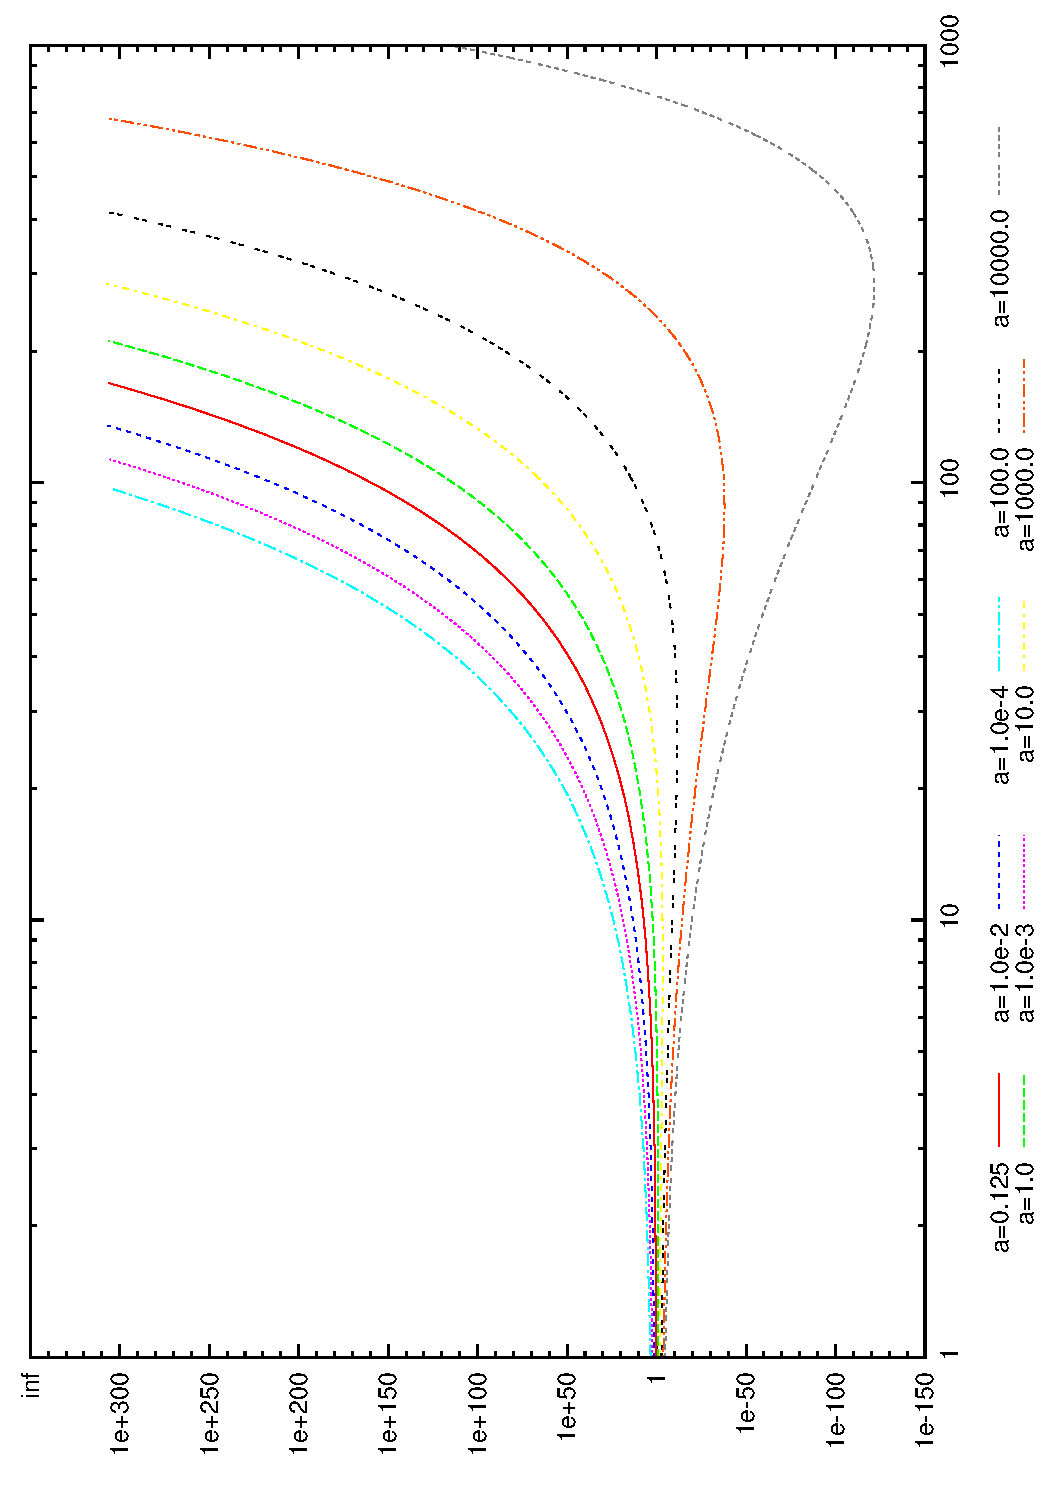
\includegraphics[angle=270,width=\the\textwidth]{../img/koeff.pdf}
  \caption[Koeffizienten in abhängigkeit von $a$]
   {Hier sind die Beträge der Koeffizienten für unterschiedliche $a$ 
    angetragen.}
\end{figure}

% vim: set ft=tex :
